\subsection{Chunked data streaming}

The Erlang NetInf NRS includes two different ways to stream chunked data. The first is the modified version of NetInf that removes the overhead of publishing each chunk to the NRS. The other implementation uses pure NetInf to publish each chunk. Both of them use an HTML5 interface to playback the stream. 

%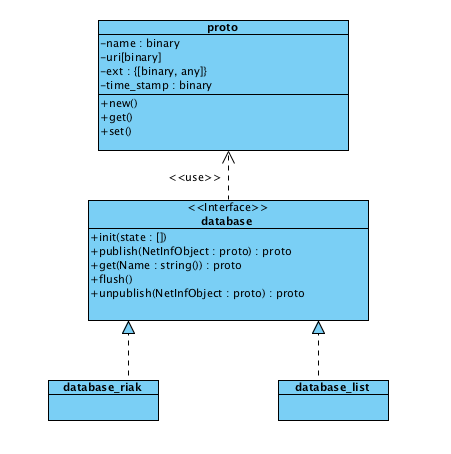
\includegraphics[scale=0.5]{./img/database_api.png}

\subsubsection{Content dispatcher}

To be able to transfer the chunks to the local HTML5 interface a content dispatcher service was added. The difference is that the content dispatcher service serve the NDOs' octects directly through HTTP, that is without the multi-part response as done in the HTTP CL. The module for this is the \textit{nn\_ct\_handler}. This service is spawned when the NRS system starts and runs on port 8078. To request the octects of the NDO \textit{ni:///sha-256-64;abc} pass the url:
\begin{verbatim}
http://localhost:8078/octets/ni%3A%2F%2F%2Fsha-256-64%3Babc 
\end{verbatim}

\subsubsection{Stream handler}
The stream handler module \textit{nn\_stream\_handler} handles fetching and polling of chunked octets between different NetInf nodes. When a user node subscribe to a stream 
In both streaming implementations the logic for fetching the chunks is to shuffle the list of available locators and fetch all available chunks in the ICN. When there are no more chunks, the stream handler retries on a regular interval. After a defined number of retries it will finally terminate itself.  

\subsubsection{HTTP client}
The module \textit{nn\_http\_client\_handler} module is used top serve the HTML5 interface for NetInf Get, Publish and Search requests. It forwards these requests to the local NRS. The client is run on port 8079. The different interfaces that can be seen are

The interface for regular NetInf interaction, located at 
http://localhost:8079/

The modified streaming, located at
http://localhost:8079/stream

The pure streaming, located at
http://localhost:8079/streampure

Other than above viewable URIs there are a couple of other request that can be used to interact with the system. 

Subscribe to a modified chunked stream, http://localhost:8079/subscribe

Subscribe to a pure NetInf stream, http://localhost:8079/subscribe/search\_and\_get


\subsubsection{HTML5 interfaces}
To combine the video chunks, two HTML5 video elements are used to pre-cache the chunks through the transfer dispatcher. This is done by alternating the visibility and playback of the two elements with JavaScript. With this method of playback the chunks looks like one continuous stream. 
To make the usability of the interface smoother, some asynchronous network request are used to communicate with the HTTP client.
To the right of the interfaces it is possible to see the current state of the local NRS. 

\subsubsection{Difference between implementations}
